\documentclass[11pt]{article}
\usepackage{fullpage}
\usepackage[english]{babel} %frenchb]{babel}
\usepackage[usenames]{color} %pour la couleur
\usepackage{amssymb} %maths
\usepackage{amsmath} %maths
\usepackage{mathabx}
\usepackage[latin1]{inputenc} %utile pour taper directement les caractères accentués
\usepackage[T1]{fontenc} 
\usepackage{hyperref}
\newtheorem{theorem}{Th�or�me}[section]
\newtheorem{lemma}{Lemme}[section]
\newtheorem{corollary}{Corollaire}[section]
\newtheorem{example}[theorem]{Exemple}
\newtheorem{definition}[theorem]{D�finition}
\usepackage[]{amsmath, amssymb, tabularx}
\usepackage{eurosym}
%\include{MacrosJEP}
\usepackage{float}

\input xy
\xyoption{all}

\usepackage{tikz} 
\usetikzlibrary{automata,calc}

\usepackage{xspace}

\setcounter{MaxMatrixCols}{15}

\title{C++ Project \\ MSc 203 \\ University Paris Dauphine}

\author{Thibaut JEREBITZ \\ Florian PERIGNE \\ Valentin ROCHEREAU}

\begin{document}
%%%%%%%%%%%%%%%%%%%%%%%%%%%%%%%%%%%%%%%%%%%%%%%%%%%%%


%%%%%%%%%%%%%%%%%%%%%%%%%%%%%%%%%%%%%%%%%%%%%%%%%%%%%
\begin{titlepage}

\begin{figure}[H]
\begin{center}

\includegraphics[height=3cm]{Logo_Dauphine.png}
\end{center}
\end{figure}

\vspace*{\fill}

\centering \Huge
MSc 203 \\ 
University Paris Dauphine\\
\vspace*{\fill}
\normalsize

\begin{center}
\LARGE
\textbf{C++ Project }\\  
\end{center}
\normalsize

\vspace*{\fill}

\textbf{Thibaut JEREBITZ \\ Florian PERIGNE \\ Valentin ROCHEREAU}




\end{titlepage}
%%%%%%%%%%%%%%%%%%%%%%%%%%%%%%%%%%%%%%%%%%%%%%%%%%%%%%%
%%%%%%%%%%%%%%%%%%%%%%%%%%%%%%%%%%%%%%%%%%%%%%%%%%%%%%%
\maketitle

\vspace*{\fill}

\begin{abstract} 

\begin{center}
The goal of the project is to solve the Black Scholes PDE. \\
In this document, we develop the mathematics needed to implement a C++ code to solve the PDE.
\end{center}

\end{abstract}
\vspace*{\fill}

\addcontentsline{toc}{section}{Abstract}
%%%%%%%%%%%%%%%%%%%%%%%%%%%%%%%%%%%%%%%%%%%%%%%%%%%%%%%
\newpage
\maketitle

\renewcommand{\contentsname}{Outlines} 
\tableofcontents


%%%%%%%%%%%%%%%%%%%%%%%%%%%%%%%%%%%%%%%%%%%%%%%%%%%%%%%
%%%%%%%%%%%%%%%%%%%%%%%%%%%%%%%%%%%%%%%%%%%%%%%%%%%%%%%
\newpage
\section{Introduction} 

The price of a European option satitisfies the \textit{Black Scholes equation}
\begin{gather*}
0 = \frac{\partial f}{\partial t}(s, t) + \frac{1}{2}\sigma^2 s^2 \frac{\partial^2 f}{\partial s^2}(s, t)
+ r s \frac{\partial f}{\partial s}(s, t) - rf(s, t)
\end{gather*}
with the final condition $f(s, T) = V(s)$ where $V(s)$ is the payout.\\

Applying the variable change $x = log(s)$ yields :
\begin{gather*}
\frac{\partial f}{\partial t}(x, t) = -\frac{1}{2}\sigma^2 \frac{\partial^2 f}{\partial x^2}(x, t)
+ (\frac{1}{2}\sigma^2 - r) \frac{\partial f}{\partial x}(x, t) + rf(x, t)
\end{gather*}

with the final condition $f(x, T) = V(x) = V(e^s)$.\\

A common method to solve this PDE is to use finite differences to approximate the derivatives and then
solve the equation on a discrete mesh.\\

When developping the different formula, we will have to set boundaries conditions for the points on the border of the mesh. We will develop two possible solutions to set these conditions : 
\begin{itemize}
	\item Dirichlet method (part \ref{Dpart} )
	\item Neumann method (part \ref{Npart} )
\end{itemize}


%%%%%%%%%%%%%%%%%%%%%%%%%%%%%%%%%%%%%%%%%%%%%%%%%%%%%%%
%%%%%%%%%%%%%%%%%%%%%%%%%%%%%%%%%%%%%%%%%%%%%%%%%%%%%%%
\newpage
\section{Dirichlet }\label{Dpart}

\indent $ \forall  n \in  \ldbrack  1 , N  \rdbrack , \forall  i \in  \ldbrack  0,x_{max}  \rdbrack, $\\

\begin{align}
f_{i}^{n} &= f(t_{n},x_{i}) \\
\frac{f_{i}^{n+1} - f_{i}^{n}}{dt} &= \theta L_{i}^{n}  + (1-\theta) L_{i}^{n+1} 
\end{align}

%\begin{align}
%\begin{split}
%f_{i}^{n+1} \left( \frac{1}{dt} - \frac{\sigma^2}{dx^2} (1- \theta) - r (1 - \theta) \right)  &+
%f_{i+1}^{n+1} \left( \frac{\sigma^2}{2dx^2} (1- \theta) -  (\frac{\sigma^2}{2}- r) (1- \theta) \frac{1}{2dx} \right)  \\
%+ f_{i-1}^{n+1} \left( \frac{\sigma^2}{2dx^2} (1- \theta) +  (\frac{\sigma^2}{2}- r) (1- \theta) \frac{1}{2dx} \right)  &=
%f_{i}^{n} \left( \frac{1}{dt} + \frac{\theta \sigma^2}{dx^2} + r \theta  \right) \\
%+ f_{i+1}^{n} \left( -\theta \frac{\sigma^2}{2dx^2} +  (\frac{\sigma^2}{2}- r) \theta \frac{1}{2dx} \right) 
%&+ f_{i-1}^{n} \left( -\theta \frac{\sigma^2}{2dx^2} - (\frac{\sigma^2}{2}- r) \theta \frac{1}{2dx} \right)  
%\end{split}\\
% f_{i}^{n+1} A_{1}^{(1-\theta)} +f_{i+1}^{n+1} B_{-}^{(1-\theta)}  +f_{i-1}^{n+1} B_{+}^{(1-\theta)} &=
% f_{i}^{n} A_{2}^{\theta} - f_{i+1}^{n} B_{-}^{\theta}  -f_{i-1}^{n} B_{+}^{\theta} 
% \end{align}
 
Let  $ A_{1}^{(1-\theta)}, B_{-}^{(1-\theta)}, B_{+}^{(1-\theta)}, A_{2}^{\theta}, B_{-}^{\theta} $ and $ B_{+}^{\theta} $ take the following values :
 
\begin{align}
\begin{split}
A_{1}^{(1-\theta)} &= \frac{1}{dt} - \frac{\sigma^2}{dx^2} (1- \theta) - r (1 - \theta)   \\
B_{-}^{(1-\theta)} &= \frac{\sigma^2}{2dx^2} (1- \theta) -  (\frac{\sigma^2}{2}- r) (1- \theta) \frac{1}{2dx}  \\
B_{+}^{(1-\theta)} &= \frac{\sigma^2}{2dx^2} (1- \theta) +  (\frac{\sigma^2}{2}- r) (1- \theta) \frac{1}{2dx} \\
A_{2}^{\theta} &=  \frac{1}{dt} + \frac{\theta \sigma^2}{dx^2} + r \theta  \\
B_{-}^{\theta} &= -\theta \frac{\sigma^2}{2dx^2} +  (\frac{\sigma^2}{2}- r) \theta \frac{1}{2dx} \\ 
B_{+}^{\theta} &= -\theta \frac{\sigma^2}{2dx^2} - (\frac{\sigma^2}{2}- r) \theta \frac{1}{2dx}   
\end{split}
\end{align}

Then we obtain :

\begin{align} \label{formula0}
 f_{i}^{n+1} A_{1}^{(1-\theta)} +f_{i+1}^{n+1} B_{-}^{(1-\theta)}  +f_{i-1}^{n+1} B_{+}^{(1-\theta)} &=
 f_{i}^{n} A_{2}^{\theta} - f_{i+1}^{n} B_{-}^{\theta}  -f_{i-1}^{n} B_{+}^{\theta} 
 \end{align}
 
 The previous formula gives us the following matrix system :
 
\begin{align}
\begin{split}
\label{matsys}
 \begin{pmatrix}
1 & 0 & 0 & 0 & 0 & \cdots & 0 & 0\\
B_{+}^{(1-\theta)} & A_{1}^{(1-\theta)} & B_{-}^{(1-\theta)} & 0 & 0 & \cdots & 0 & 0\\
0 & B_{+}^{(1-\theta)} & A_{1}^{(1-\theta)} & B_{-}^{(1-\theta)} & 0 & \cdots & 0 & 0 \\
\vdots& \vdots & \vdots & \vdots & \vdots & \ddots & \vdots & \vdots \\
0& 0 & 0 & 0 & 0 & \cdots & 0 & 1 
\end{pmatrix}
 \begin{pmatrix}
f_{0}^{n+1}\\
f_{1}^{n+1}\\
\vdots \\
f_{x_{max}-1}^{n+1}\\
f_{x_{max}}^{n+1}\\
\end{pmatrix}
\\ = 
 \begin{pmatrix}
e^{r dt} & 0 & 0 & 0 & 0 & \cdots & 0 & 0\\
-B_{+}^{\theta} & A_{2}^{\theta} & -B_{-}^{\theta} & 0 & 0 & \cdots & 0 & 0\\
0 & -B_{+}^{\theta} & A_{2}^{\theta} & -B_{-}^{\theta} & 0 & \cdots & 0 & 0 \\
\vdots& \vdots & \vdots & \vdots & \vdots & \ddots & \vdots & \vdots \\
0& 0 & 0 & 0 & 0 & \cdots & 0 & e^{r dt} 
\end{pmatrix}
 \begin{pmatrix}
f_{0}^{n}\\
f_{1}^{n}\\
\vdots \\
f_{x_{max}-1}^{n}\\
f_{x_{max}}^{n}\\
\end{pmatrix}
\end{split}
\end{align}

The previous system (equation \ref{matsys}) is equivalent to :
 \begin{align}
 A f^{n+1} &= B f^{n}
 \end{align}

To solve this matrix system, we use Thomas algorithm. This algorithm is used to solve matrix systems with tridiagonal matrix.
For such systems, the solution can be obtained in $O(n)$ operations instead of $O(n^{3})$ required by Gaussian elimination.
To see the complete method : \href{https://en.wikipedia.org/wiki/Tridiagonal_matrix_algorithm}{Wikipedia Thomas Algorithm.}

%%%%%%%%%%%%%%%%%%%%%%%%%%%%%%%%%%%%%%%%%%%%%%%%%%%%%%%
%%%%%%%%%%%%%%%%%%%%%%%%%%%%%%%%%%%%%%%%%%%%%%%%%%%%%%%
\newpage
\section{Neumann} \label{Npart}



$
\forall  n \in  \ldbrack  1 , N  \rdbrack , \forall  i \in  \ldbrack  0,x_{max}  \rdbrack,    \\
$

\begin{align}
\frac{df}{dx} (t_{n}, x_{0}) &= k_{1} \\
\frac{df}{dx} (t_{n},x_{0}) = \frac{f_{1}^{n}-f_{0}^{n}}{dx} &\Leftrightarrow f_{0}^{n} = f_{1}^{n} - k_{1} dx \label{formula2} 
\end{align}
\begin{align}
\frac{df}{dx} (t_{n}, x_{x_{max}}) &= k_{2} \\
\frac{df}{dx} (t_{n},x_{x_{max}}) = \frac{f_{x_{max}}^{n}-f_{x_{max}-1}^{n}}{dx} &\Leftrightarrow f_{x_{max}}^{n} = f_{x_{max}-1}^{n} + k_{2} dx \label{formula3} 
\end{align}

Using the same formula (equation \ref{formula0}):
\begin{align} \label{formula1}
 f_{i}^{n+1} A_{1}^{(1-\theta)} +f_{i+1}^{n+1} B_{-}^{(1-\theta)}  +f_{i-1}^{n+1} B_{+}^{(1-\theta)} &=
 f_{i}^{n} A_{2}^{\theta} - f_{i+1}^{n} B_{-}^{\theta}  -f_{i-1}^{n} B_{+}^{\theta} 
 \end{align}
 
 Taking the left part of the equation \ref{formula1}, and using equation \ref{formula2} we have :
 
 \begin{align} 
 f_{i}^{n+1} A_{1}^{(1-\theta)} +f_{i+1}^{n+1} B_{-}^{(1-\theta)}  +f_{i-1}^{n+1} B_{+}^{(1-\theta)} &=
 f_{1}^{n} A_{2}^{\theta} - f_{2}^{n} B_{-}^{\theta} -  (f_{1}^{n} - k_{1} dx) B_{+}^{\theta} \\
&=  f_{1}^{n} (A_{2}^{\theta} - B_{+}^{\theta} ) - f_{2}^{n} B_{-}^{\theta} + k_{1} B_{+}^{\theta} dx
\end{align}
 
Taking the right part of the equation \ref{formula1}, and using equation \ref{formula3} we have :

 \begin{align} 
 f_{i}^{n} A_{2}^{\theta} - f_{i+1}^{n} B_{-}^{\theta}  -f_{i-1}^{n} B_{+}^{\theta}  &=
f_{x_{max}-1}^{n} A_{2}^{\theta} - f_{x_{max}}^{n} B_{-}^{\theta} -f_{x_{max}-2}^{n} B_{+}^{\theta} \\
&=  f_{x_{max}-1}^{n} (A_{2}^{\theta} - B_{-}^{\theta} ) - k_{2} B_{-}^{\theta} dx -  f_{x_{max}-2}^{n} B_{+}^{\theta} 
 \end{align}
 
  The previous formulas give us the following matrix system :
  
\begin{align}
\begin{split}
 \begin{pmatrix}
-\frac{1}{dx} & \frac{1}{dx} & 0 & 0 & 0 & \cdots & 0 & 0 & 0 & 0\\
B_{+}^{(1-\theta)} & A_{1}^{(1-\theta)} & B_{-}^{(1-\theta)} & 0 & 0 & \cdots & 0 & 0 & 0 & 0\\
0 & B_{+}^{(1-\theta)} & A_{1}^{(1-\theta)} & B_{-}^{(1-\theta)} & 0 & \cdots & 0 & 0 & 0 & 0 \\
\vdots& \vdots & \vdots & \vdots & \vdots & \ddots & \vdots & \vdots & \vdots & \vdots & \vdots \\
0 & 0 & 0 & 0 & 0 & \cdots & 0 & B_{+}^{(1-\theta)} & A_{1}^{(1-\theta)} & B_{-}^{(1-\theta)}  \\
0& 0 & 0 & 0 & 0 & \cdots & 0 & 0 & -\frac{1}{dx} & \frac{1}{dx}
\end{pmatrix}
 \begin{pmatrix}
f_{0}^{n+1}\\
f_{1}^{n+1}\\
\vdots \\
f_{x_{max}-1}^{n+1}\\
f_{x_{max}}^{n+1}\\
\end{pmatrix}
\\ =
 \begin{pmatrix}
1 & 0 & 0 & 0 & 0 & \cdots & 0 & 0 & 0 & 0 & 0 \\
B_{+}^{\theta} dx & A_{2}^{\theta}-B_{+}^{\theta}  & -B_{-}^{\theta} & 0 & 0 & \cdots & 0 & 0 & 0 & 0 & 0\\
0 & -B_{+}^{\theta} & A_{2}^{\theta} & -B_{-}^{\theta} & 0 & \cdots & 0 & 0 & 0 & 0 & 0 \\
\vdots& \vdots & \vdots & \vdots  & \vdots  & \ddots & \vdots & \vdots & \vdots & \vdots  & \vdots  \\
0& 0 & 0 & 0 & 0 & \cdots & 0 & -B_{+}^{\theta} & A_{2}^{\theta} & -B_{-}^{\theta} & 0 \\
0 & 0 & 0 & 0 & 0 & \ldots & 0 & 0 & -B_{+}^{\theta} & A_{2}^{\theta}-B_{-}^{\theta} & -B_{-}^{\theta}dx \\
0& 0 & 0 & 0 & 0 & \cdots & 0 & 0 & 0 & 0 & 1
\end{pmatrix}
 \begin{pmatrix}
k_{1}\\
f_{1}^{n}\\
\vdots \\
f_{x_{max}-1}^{n}\\
k_{2}\\
\end{pmatrix}
\end{split}
\end{align}



%%%%%%%%%%%%%%%%%%%%%%%%%%%%%%%%%%%%%%%%%%%%%%%%%%%%%%%
%%%%%%%%%%%%%%%%%%%%%%%%%%%%%%%%%%%%%%%%%%%%%%%%%%%%%%%
\newpage
\section{Userguide} 

\subsection{Volatility and Rates inputs}
Our program offers the possibility to the user to input the volatility matrix and the rates vector in an excel (csv) file. To do so, the program will ask the user if he wants to use this feature (see figure \ref{terminal1}). If the user answers "yes" (y) then the program creates two .csv files to be completed by the user. One for the volatility and the other one for the rates. To input its parameters, the user can open the .csv file in excel, and convert the column A "from text to columns". User will find an empty matrix with the X in lines (all spot prices) and Y in columns (all the times considered). Once saved the user continues to run the program by pressing "ENTER".\\
User can choose to change the separators in the $.csv$ files.

\begin{figure}[H]
\begin{center}
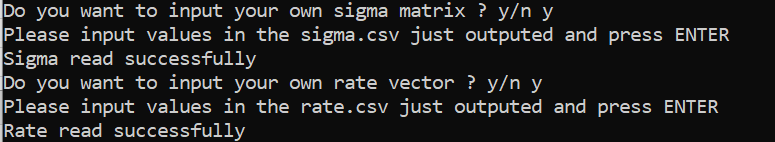
\includegraphics[height=3cm]{terminal.png}
\caption{Options available}\label{terminal1}
\end{center}
\end{figure}

\subsection{Payoff function}

The function payoff takes three arguments : a name for the chosen payoff, a vector (strikes) and a function. All these parameters are optional. If the user doesn't enter anything, the payoff will be $g=S$. The user can enter a name of payoff recognised by the program. The registered payoffs are : "Call", "Put", "Call Spread", "Put Spread", "Straddle", "Strangle". Once the payoff's name chosen, the user has to enter a parameter for the strike(s) of the payoff chosen. If several ones are entered, the program will only take into account the first one for a single strike strategy ("Call", "Put"). For multiple strike strategies ("Call Spread", "Put Spread", "Straddle", "Strangle") the user has to enter the strikes from the smallest to the biggest.\\
If the user wants to generate a customised payoff, he has to input a different name (one not recognised by the program). Then enter the different strikes and finally the function of the payoff.






\end{document}
